\label{developmentIntroduction}
The aim of the development was to categorize the scraped pages into categories. This was to be done depending on the content of the pages. The second goal was to provide a way to observe the structure of the pages, links between them, and categories. One of the partner requirements was for the application to function on a UNIX system. Another requirement was a user friendly UI. Also, the option of retrieving all the available information about the pages was demanded. 

This chapter describes the design and implementation of the application which is composed of a representational state transfer (REST) application program interface (API) and a front-end (FE) web application. 

\section{API}
The scraped pages of the dark-web were stored in \textit{ElasticSearch}. We created a back-end application (BE) in order to perform various operations on the data-set before sending it to the FE. Such operations involve resource intensive processing of large volumes of data, and caching. We decided to create a Python BE. The reason behind this decision was the requirement for the application to function on a UNIX system. Other reasons are described in subsection~\ref{technologyOverwiew}. The requirements for the BE was the categorization of the nodes along with their division into groups. The groups were either represented by nodes of the same category or communities. The BE also needed functionality to return details for specific pages or groups if requested.
\subsection{Technology overview}
\label{technologyOverwiew}
\textit{Python} is a widely used interpreted programming language known for readability and portability \cite{aboutPython}. Python is open-source and is considered to have an extensive documentation and community available. 

Python is popular in the science community because it is easy to learn and has simple syntax. There is therefore a great amount of useful libraries for research purposes such as \textit{NetworkX}\footnote{A library used for creating and working with graphs.} \cite{networkX} or \textit{cylouvain}\footnote{A library with a fast implementation of LA.} \cite{cylouvain} because of this.  
As we wanted to follow the REST architecture we decided to make use of the \textit{Django} framework \cite{meetDjango}. It is responsible for tasks such as running the server or managing web requests. Another advantage of Django is its \textit{Django REST framework} (DRF). DRF offers a convenient way for creating restful endpoints and responses \cite{djangoRest}. Both frameworks are open-source with helpful documentation and community. 

We had to solve performance issues. It took approximately 30 minutes to retrieve and categorize about 220,000 pages from the database and circa xxx seconds to divide such a response into communities. We considered this wait time to be too long. Therefore we decided to cache the data of the first response. For that purpose \textit{Redis} \cite{redis} was used. It is an open-source solution which we used as a key-value store. It supports basic data structures\footnote{Simple structures, e.g. strings, numbers or sets.} as values, but not custom objects. Since the API uses custom objects for \textit{communities}, \textit{pages} and \textit{links}, an object serializer was leveraged along with Redis. We decided not to write our own but to utilise the Python \textit{pickle} module\footnote{A module used for converting Python objects to streams of bytes and vice versa.} \cite{pickle} (pickle). The reason behind this decision was the simplicity of pickle. Pickle also fulfilled all our needs for serializing. Specifically the serialization or deserialization of data in the form of the previously mentioned models for Redis to store in an acceptable time. Pickle took xxx seconds to serialize xxx pages. The deserialization of the same number of pages took xxx seconds.

\section{Front-end}
For users to be able to see the data acquired from the BE in a reasonable way a FE application was created. The goal of this FE was to visualize the scraped pages in a graph. The pages or communities, and links from the BE were to depict nodes, and links of the graph respectively. The category of the pages or communities was to be readable from the graph. Additional information about the nodes needed to be displayed or retrieved on demand.

\subsection{User interface}
We designed the UI the following way. 

After the application is loaded the UI is composed of a \textit{header} with the name of the application \textit{Dark web categorization}, a \textit{loader} and a \textit{sidebar} on the right hand side. The \textit{sidebar} contains several \textit{input fields} and \textit{buttons} in a column as can be viewed in Figure \ref{zeroLevelGraphBasic}. At the very top of the \textit{sidebar} a \textit{drop-down button} (DD) is present. 

The DD sets the mode according to which the pages are grouped into communities. There are two modes available, \textit{link-mode} and \textit{category-mode}. If \textit{link-mode} is selected, the pages are divided by the LA\ref{louvainAlgorithm} depending on the connections between them only. If \textit{category-mode} is selected, the pages are divided into groups by categories. The pages in the groups are further divided into communities according to links between them, as if in \textit{link-mode}. 

 An \textit{input field} with a \textit{submit button} was placed underneath the DD for the purpose of filtering nodes according to a search phrase. The last element shown is an indicator of the current level - how many times the user zoomed into a community. The indicator has a \textit{zoom-out button} placed next to it.
\begin{figure}[ht!]
  \centering
  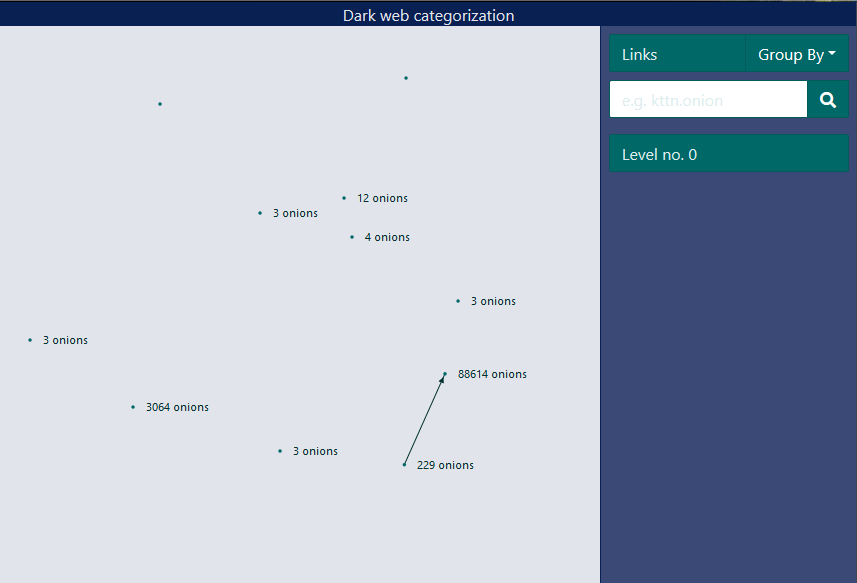
\includegraphics[width=\textwidth]{Images/ZeroLevelGraphBasic.png}
  \caption{The basic view of the app with a selected community and its details.}
  \label{zeroLevelGraphBasic}
\end{figure} 

The moment the data is retrieved from the BE the \textit{loader} gets replaced for a graph. The graph-nodes represent either the communities the pages are partitioned into or the pages themselves.  If the graph contains any isolated nodes (isolates) a \textit{mock-community} is displayed containing all isolates. This community cannot be zoomed into. A community node is depicted as a \textit{pie chart}. The individual sectors of the \textit{pie chart} represent the categories of the pages belonging into the community [picture]. A single page is represented as a square [picture] because it was otherwise difficult to differentiate between a single page and a small community of only one category. The colour of the square corresponds to the category of the page. It is possible for a level to depict communities and pages at once. The links between the nodes visualize the links between pages or communities. 

After single-clicking a node additional information is exampled in the \textit{sidebar}.The details vary depending on whether the node is representing a community or a single page.  
The details of an individual page are as follows: 
\begin {description}
	\item [Url] which also serves as a unique identificator of the page. 
	\item [Category] of the page. Each page belongs to exactly one category.
	\item[Links] to other pages displayed as a list of url addresses. There are up to ten links visible in the sidebar. The remaining links, if any, are downloadable in a text file. 
	\item[Content] of the page if it is available. If the content is too long to be disclosed in the sidebar it is downloadable in a text file.
\end{description}
[picture]

The details of a community consist of  grouped information of its pages and include the following:
\begin {description}
	\item [Category composition] which is aggregated from the categories of all the pages of the community. Each category is represented by its name and the percentage of its relevance in the community.
	\item [Page url] addresses (urls) of members belonging into the community. There are up to ten urls visible in the sidebar. The remaining urls, if any, are downloadable in a text file. 
	\item[Urls count]represents the number of all the pages belonging into the community. 
\end{description}
[picture]

In case of the need of further information a link, also present in the \textit{sidebar}, can be clicked. If clicked, a \textit{pop-up window} with detail-options is displayed. Details may include the \textit{title}, \textit{category}, \textit{links} and \textit{page-content}, depending on the user's selection. \textit{Urls} of the pages are present by default. After selecting the needed options and clicking the \textit{download button}, a \textit{text file} with the desired information is downloaded. The page or community-members with their details are depicted in JSON format. This functionality was required for the scenario of the user needing to download all available data about members of a specific community.

A graph node representing a community can be double clicked. After doing so, a new graph is shown. The data of this graph consists of the members of the clicked community. We call this process \textit{zooming}. In case the parent community contains too many sub-communities, it is displayed as a single community-node. The zooming-in or -out of communities adjusts the \textit{zoom-level}. This level is represented by a number and is visible below the \textit{node-filter}. If the current zoom level is more than zero, i.e. at least one community-node was double clicked, a button for zooming out appears next to the \textit{level indicator}. It is shown in Figure \ref{levelIndicatorWithButton}.
\begin{figure}[ht!]
  \centering
  
\includegraphics{Images/levelIndicatorWithButton.png}
  \caption{The level indicator with the zoom-out button. After the zoom-out button is clicked, the user is shown the communities of the previous level.}
  \label{levelIndicatorWithButton}
\end{figure} 

If further zooming is not possible, the user reached the maximum level. Each community may have a different maximum level, depending on the number of its pages and its structure.

\subsection{Technology overview}
\textit{JavaScript} \cite{javaScript} (JS) is the most favoured programming language used for creating web applications \cite{jsGithut}. It is an interpreted language supported by all modern browsers. It is open-source and as such disposes of a considerable community with convenient documentation. JS is not strongly typed and the code might therefore be complicated to read or navigate. For this reason the FE was written in \textit{TypeScript} (TS) \cite{typeScript} which is a superset of JS with the advantage of being typed. There is a significant number of tools and libraries for implementing user interfaces (UI) in a clean and timely manner created for both JS and TS. One of such tools is the framework \textit{React.js} \cite{react} (React). React is one of the most favoured JS frameworks \cite{reactPopularity}. The advantages of using React are readable code and improved performance by managing the re-rendering of page elements.

To achieve a satisfying UX the app needed to be interactive and obtain new or modified data frequently. Repeated requests to the BE would mean longer wait time for the user. However, a proper mechanism for data-storing would present a convenient solution to this issue and make the requests unnecessary. A JS library which handles the app state and works well with TS and React is called \textit{Redux.js} \cite{redux} (Redux). Redux is a single store approach. This ensures easy hydration\footnote{The process of an object being provided with information}. Redux also provides a custom set of TS typings and provides the developers with easy to use debugging tools. Another advantage of this library is the documentation.

The visualization of the web graph alone was realized using the \textit{react-d3-graph} library \cite{reactD3Graph} (RD3). RD3 is 
an implementation of the library D3.js \cite{d3} made more convenient for the use with React.js. 

\subsection{Implementation}
The FE project consists of three folders and several configuration files. The folder \texttt{node\_modules} contains imported libraries including \textit{React.js}, \textit{Redux} or \textit{d3}. The next folder named \texttt{public} encloses a \textit{.ico} file\footnote {A picture with the dimensions 16x16 pixels used by the browser to represent the web page or application. It is usually displayed in the tab in which the application is opened.} and a html file which is the default entry point when the application is started. The last folder \texttt{src} contains the source code itself. 

As previously mentioned, the FE is written in TS which has the advantage of readability and easy navigation. There are, however, also disadvantages. One of them is the need of a TS file with the types (typing) for every used library. Typings for popular libraries are often downloadable as modules. If a library has no ready-to-download typings own ones need to be written. In our case the typings for the library \textit{react-d3-graph} were custom made. They can be found in the folder \texttt{@types/react-d3-graph}. The file \texttt{commont.d.ts} holds types used heavily across the application, e.g. \textit{Action}. Types in this file are available without importing them to all files in the project.  

Objects passed between functions also need to be typed. Those models are stored in the folder \texttt{models}. Each file contains one server-model and one client-model. The conversion between these models is conducted in specific helper functions. The advantage of this approach is the independence of client-models from the BE models.

The visual aspect is implemented using Less \cite{less} which is a language extending CSS with improvements such as the possibility of using variables. The Less classes are divided into files depending on the element they are meant to modify. These files were placed into the folder \texttt{styles}. 

The remaining folders each represent a different part of the UI. The structure of their sub-folders is similar. Therefore it is sufficient to describe them as a whole. Folders named \texttt{utils} contain files with helper functions such as converters between server and client models. \texttt{Constants} contains folders with string constants or simple functions which return a string depending on the input. The rest of the folders represent some part of the Redux framework. 

The most basic files which only include string constants are situated in the folders named \texttt{actionTypes}.  These are utilised as action types in actions. An action is a simple objects containing a type and an optional payload. Actions themselves are returned by action creators (AC). AC are functions returning an action and can be found in folders called \texttt{actions}. They can be as simple as those present in the file \texttt{nodesActionCreators.ts}. But they can be more complicated such as the AC \texttt{fetchNodes.ts} and dispatch multiple simple ACs. The purpose of an AC is to be injected into \hyperlink{reducers}{reducers}, i.e. dispatch them.

\texttt{fetchNodes} and the folder it is placed in share the same name. For easier testing purposes the main logic of this AC is put into a function which receives the simple ACs as dependencies. When this AC is called it first dispatches a simple AC to indicate the fetching has begun. After that an identificator (id) is created. This id is later used to create an error object in case of failure. Next, the fetching itself begins. The fetching in \texttt{fetchNodes} is realized with the library \textit{isomorphic-fetch}. The fetch function of this library expects the first argument to be the url address of the resource. The second argument is an object describing further details of the request and is optional. Such an object may contain the request method, headers or the payload. If the request does not result in error the response status is checked. After the fetching is complete a success AC with the acquired response is dispatched. If an error is caught during the fetching a failure AC is dispatched. The payload of this AC is an error-object with the id and error message if any.

The dispatching of actions enables the changing of the state via reducers situated in the \texttt{reducers} folders. The state is a single immutabe\footnote{The object cannot be adjusted directly. Instead, a new modified object is returned and the original one stays unmodified.} object and is used in the whole application. A \hypertarget{reducers}{reducer} is a pure function\footnote{The return value of a pure function is only dependent on its input values. A pure function has no side effects.} receiving the current state and the dispatched action as its arguments. It then returns the newly computed state. A reducer creates a new state only if the type of the given action is recognized. If not, the previous state is returned unmodified. The state object received or returned by the reducer does not need to be the entire state (app-state). A reducer may be responsible for just a part of the app-state. However, the root reducer is responsible for the whole app-state.

The folders \texttt{components} contain files with React components. They define the skeleton of the UI with the specified behaviour. The folders \texttt{containers} hold files with React containers. A container is a file with access to the app-state. It is responsible for passing data to components. 

